%Copyright 2014 Jean-Philippe Eisenbarth
%This program is free software: you can 
%redistribute it and/or modify it under the terms of the GNU General Public 
%License as published by the Free Software Foundation, either version 3 of the 
%License, or (at your option) any later version.
%This program is distributed in the hope that it will be useful,but WITHOUT ANY 
%WARRANTY; without even the implied warranty of MERCHANTABILITY or FITNESS FOR A 
%PARTICULAR PURPOSE. See the GNU General Public License for more details.
%You should have received a copy of the GNU General Public License along with 
%this program.  If not, see <http://www.gnu.org/licenses/>.

%Based on the code of Yiannis Lazarides
%http://tex.stackexchange.com/questions/42602/software-requirements-specification-with-latex
%http://tex.stackexchange.com/users/963/yiannis-lazarides
%Also based on the template of Karl E. Wiegers
%http://www.se.rit.edu/~emad/teaching/slides/srs_template_sep14.pdf
%http://karlwiegers.com
\documentclass{scrreprt}
\usepackage{float}
\usepackage{placeins}
\usepackage{listings}
\usepackage{underscore}
\usepackage[bookmarks=true]{hyperref}
\usepackage[utf8]{inputenc}
\usepackage[english]{babel}
\usepackage{graphicx}
\hypersetup{
    bookmarks=false,    % show bookmarks bar?
    pdftitle={Software Requirement Specification},    % title
    pdfauthor={Trevor Sherrard},                     % author
    pdfsubject={TeX and LaTeX},                        % subject of the document
    pdfkeywords={TeX, LaTeX, graphics, images}, % list of keywords
    colorlinks=true,       % false: boxed links; true: colored links
    linkcolor=blue,       % color of internal links
    citecolor=black,       % color of links to bibliography
    filecolor=black,        % color of file links
    urlcolor=purple,        % color of external links
    linktoc=page            % only page is linked
}%
\def\myversion{1.0 }
\date{}
%\title
\usepackage{hyperref}
\begin{document}

\begin{flushright}
    \rule{16cm}{5pt}\vskip1cm
    \begin{bfseries}
        \Huge{SOFTWARE REQUIREMENTS\\ SPECIFICATION}\\
        \vspace{1.9cm}
        for\\
        \vspace{1.9cm}
        Finger Lakes Explorer ROV\\
        \vspace{1.9cm}
        \LARGE{Version \myversion approved}\\
        \vspace{1.9cm}
        Prepared by Trevor Sherrard\\
        \vspace{1.9cm}
        P20250 Tiger Sharks\\
        \vspace{1.9cm}
        \today\\
    \end{bfseries}
\end{flushright}

\tableofcontents


\chapter*{Revision History}

\begin{center}
    \begin{tabular}{|c|c|c|c|}
        \hline
	    Trevor Sherrard December 2019\\
        \hline
	    21 & 22 & 23 & 24\\
        \hline
	    31 & 32 & 33 & 34\\
        \hline
    \end{tabular}
\end{center}

\chapter{Introduction}

\section{Purpose}
The requirements outlined in this document pertain to design and implementation of software for the Finger Lakes Explorer ROV for Team P20250 of Rochester Institute of Technology's Multidisciplinary Senior Design (MSD) Program.

\section{Intended Audience and Reading Suggestions}
This document is intended for the developer(s) of the overall systems software and all invested stakeholders in the project overall. These stakeholders include (but are not limited to) the project customer Dr. Jason Kolodziej, the project guide Gerald Geravuso, and the head of the MSD program Dr. Elizabeth DeBartolo. 

\section{Project Scope}
The Finger Lakes Explorer ROV is designed to be operable by a single user for recreational underwater exploration in the Finger Lakes of Western New York State. The ROV will be able to navigate within a 20 foot radius of the launch point while operating at a depth of 100 feet. The ROV will capture a video feed (and thus still images) along with analog sensor data from pressure and temperature sensors. This data will be transmitted to the surface via a twisted pair data tether to a base station that will store this mission data in a historical context. The base station will allow the user to control the ROV via commands entered via an X-Box controller. 

\section{References}
None yet.


\chapter{Overall Description}


\section{Product Functions}
This systems has two major domains of design. Those two domains being the ROV domain and Base station domain. Each of these domains serves different functions needed for the overall systems. These two systems are linked via the tether domain. The functions for each domain can be seen in this section. 

\subsection{ROV Domain}
This domain contains all the software functionality required to maintain a bi-directional connection with the base station over the tether, collect mission data from on-board sensors and camera, and actuate motors and lights via hardware controllers due to user input.

\begin{figure}[!ht]
    \centering
    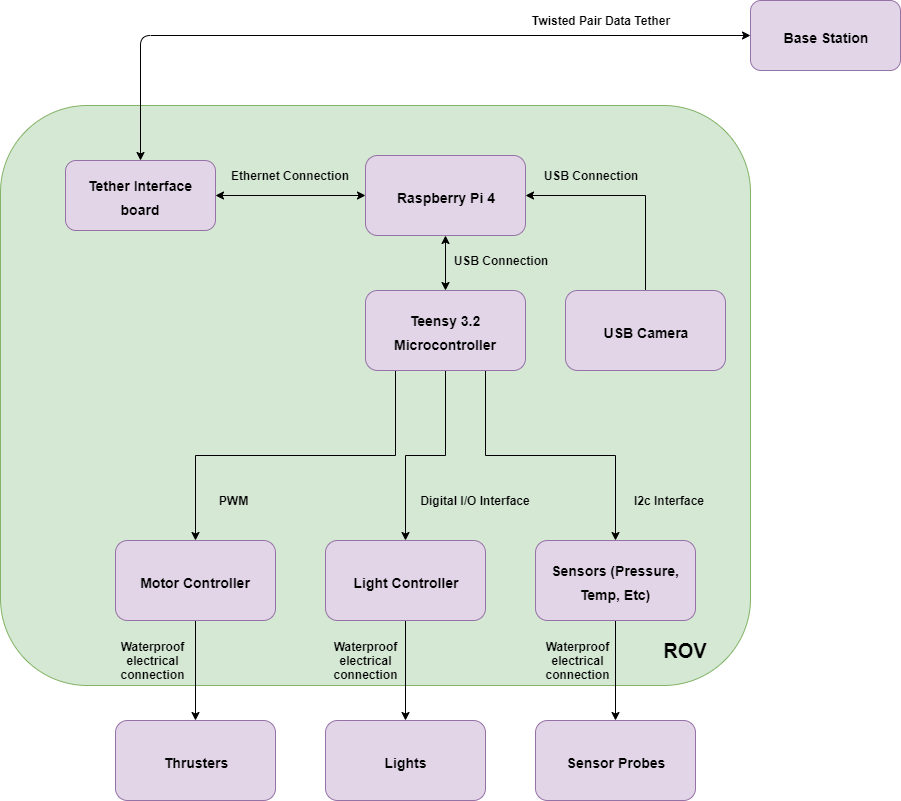
\includegraphics[scale=0.55]{ROVDomainSoftware.png}
    \caption{ROV Software Domain}
    \label{fig:ROV Software Domain}
\end{figure}
\FloatBarrier

Figure \ref{fig:ROV Software Domain} in this section depicts the overview of the ROV software domain. From the diagram above, the following software functions fall out.

\begin{itemize}
    \item ROV-Side Tether Communications Manager
    \item ROV-Camera Control Manager
    \item Micro-Controller and Raspberry Pi Serial Bridge
    \item Micro-Controller Software For Motor Control via PWM interface
    \item Micro-Controller Software For Light Control via digital I/O interface
    \item Micro-Controller Software For Sensor Data Collection via I2C interface
\end{itemize}
Later section in these documents will outline these functions in much more detail.

\subsection{Base Station Domain}
This domain contains all software functionality to maintain a bi-directional connection with the ROV over the tether interface, store mission data received from the ROV in the data archival system, start and end dive procedures, and update the HUD screen as required. 

\begin{figure}[!ht]
    \centering
    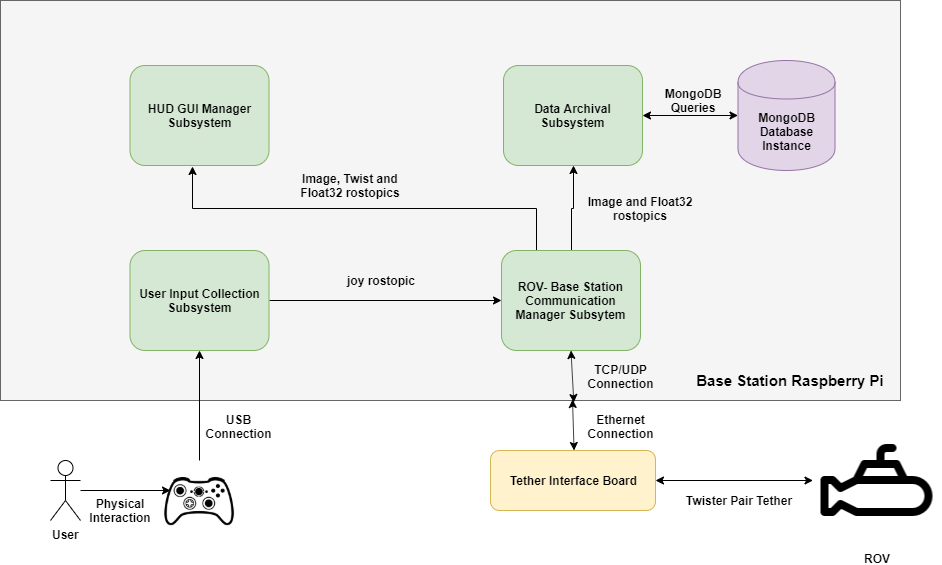
\includegraphics[scale=0.45]{BaseStationDomainSoftware.png}
    \caption{Base Station Software Domain}
    \label{fig:Base Station Software Domain}
\end{figure}
\FloatBarrier

Figure \ref{fig:Base Station Software Domain} in this section outlines the overview of the Base Station software domain. From the diagram above, the following software functions fall out.

\begin{itemize}
    \item Base Station Side Tether Communications Manager
    \item User Input Collection Manager
    \item HUD Front End Interface
    \item Data Archival Insertion Software
    \item Data Archival CSV Export Software
\end{itemize}
Later section in these documents will outline these functions in much more detail.

\section{Operating Environment}
The system's computational resources consist of two Raspberry Pi 4 single board computers and one Teensy 3.2 Micro-Controller. Both Raspberry Pi 4 devices have 4GB of available memory, and a Broadcom BCM2711B0 quad-core A72 (ARMv8-A) 64-bit processor operating at 1.5GHz. The ROV Raspberry Pi will have 16GB of hard disk space, and the base station will have 64GB of hard disk space. All Software shall be written to handle potential faults that occur from running computational resources in an real-time embedded setting.

\section{Design and Implementation Constraints}
Both Raspberry Pi devices only have 4GB of RAM and software on both base station and ROV, and thus software on both computational resources should be developed accordingly. The data archival system should be designed to interface with a MongoDB database instance. The maximum effective bandwidth over the twisted pair tether is 80 MBit/sec. Data packets being sent over the tether should be constructed and scheduled to account for this limitation. The hard disk size for the ROV Raspberry Pi is 16GB and the hard disk size for the base station hard disk size is 64GB and software on either raspberry pi must be designed within these limits.  

\section{User Documentation}
The project will be delivering all generate source code and system launch scripts upon completion of the project. Documentation of system configuration and source code as implemented will also be delivered upon project completion. A user manual for operation of ROV will be constructed and delivered with the final system prototype. 

\section{Assumptions and Dependencies}

The overall system will use ROS for message passing between the different nodes on both the ROV and base station domains. Data acquisition will be implemented through the use of a third party ROS node known as mongodb_store. This also requires the data storage database to be a MongoDB instance. The user collection software subsystem relies on a third party device driver for communicating with the Xbox controller via the base station computer. All third party source being considered for use is licensed under a free and open source software licence and thus can be used for this project's purposes. 

\chapter{External Interface Requirements}

\section{User Interfaces}
The Heads Up Display (HUD) Software System will be the main interface with the ROV operator. This interface will be developed as a multi-page react web application with interfaces to a backend containing collected mission data and live frames collected from the ROV. This interface will display live video feeds from the ROV camera. It will also display an instantaneous reading of each mission data parameter, as well as an estimated pose of the ROV in three dimensional space. The main page of the HUD interface will also have a list of recent commands run via the Xbox controller interface as well as a box to display any messages sent from the ROV to the base station. Figure \ref{fig:Main HUD Page Mockup View} in this section outlines a graphical mockup of this webpage.

\begin{figure}[!ht]
    \centering
    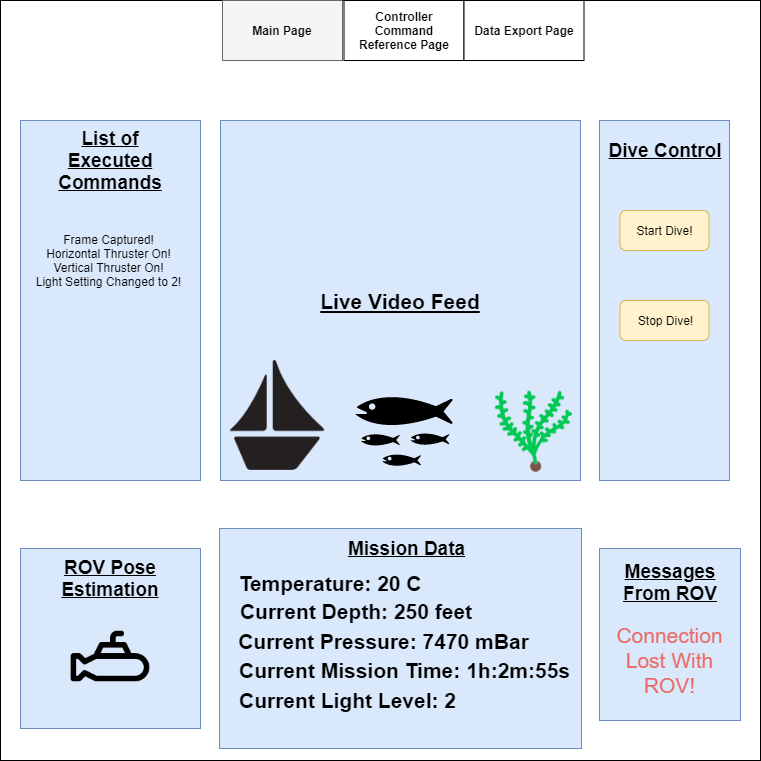
\includegraphics[scale=0.45]{MainPageHUDMockup.png}
    \caption{Main HUD Page Mockup View}
    \label{fig:Main HUD Page Mockup View}
\end{figure}
\FloatBarrier

The second page of the HUD interface will contain a reference for accessible commands able to be executed from the Xbox controller interface. This page will provide a graphical depiction of the Xbox controller to reference against the available list of commands. Figure \ref{fig:Controller Reference Page Mockup View} in this section outlines the graphical depiction of the controller reference view. 

\begin{figure}[!ht]
    \centering
    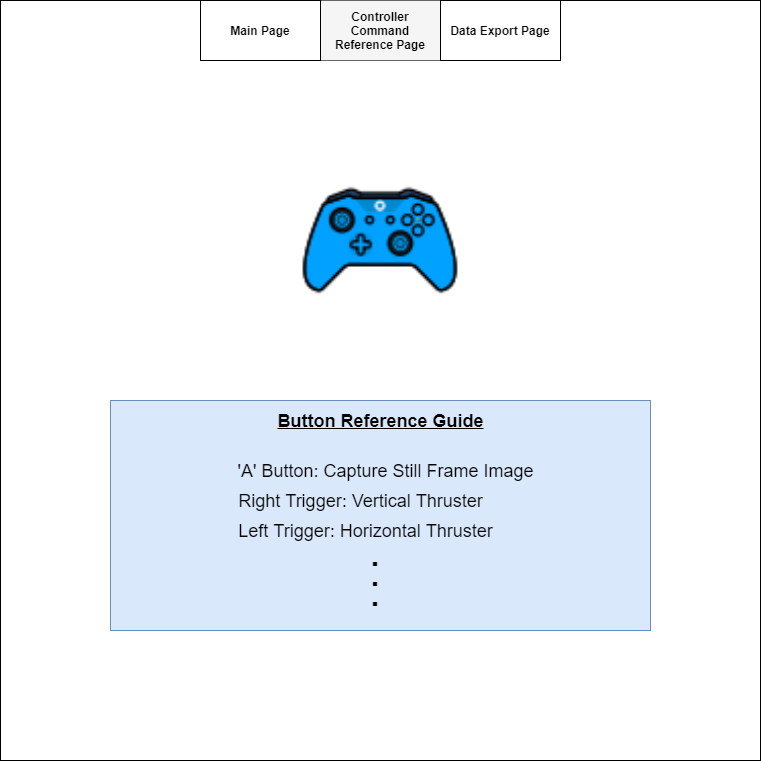
\includegraphics[scale=0.45]{ControllerReferencePageMockup.png}
    \caption{Controller Reference Page Mockup View}
    \label{fig:Controller Reference Page Mockup View}
\end{figure}
\FloatBarrier

The third page of the HUD interface will contain an interface for the exporting of mission data to a CSV file based on a datetime range. The user will select a 'to' datetime and a 'from' datetime range and all data within the MongoDB database instance that fits that range will be compiled into a CSV file on the backend server and will be downloaded through the web interface. The user can then insert a flash-drive or other portable storage media to extract this CSV file from the system. Figure \ref{fig:Data Export Page Mockup View} in this section outlines the graphical depiction of the data export page view.

\begin{figure}[!ht]
    \centering
    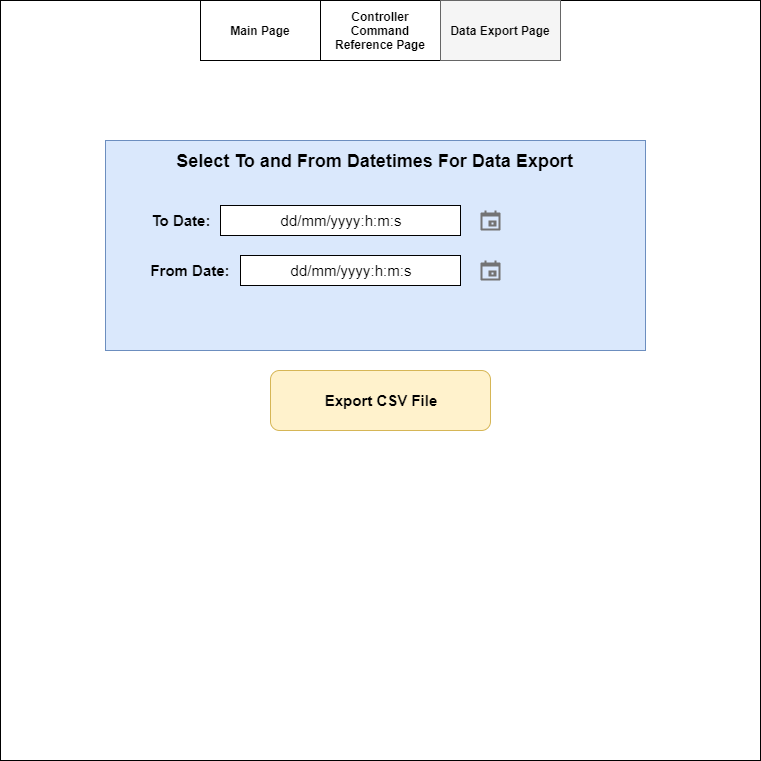
\includegraphics[scale=0.45]{DataExportPageMockup.png}
    \caption{Data Export Page Mockup View}
    \label{fig:Data Export Page Mockup View}
\end{figure}
\FloatBarrier


\section{Hardware Interfaces}
The main hardware interface that interfaces with users is the Xbox controller. This will communicate with the base station computer via a third party device driver from Microsoft. All sensors on-board the ROV will interface with the Teensy micro-controller via an I2C interface. The Teensy will also communicate with the motor controllers and lighting controller via PWM and digital I/O interfaces, respectively. The ROV and Base station software domains are coupled via the tether hardware interface for bi-directional data communication. Figure \ref{fig:Base Station Software Domain} depicts the hardware interfaces needed for the ROV software domain. The only major hardware interface on the base station side is the tether interface board to couple digital communication over the tether to the base-station Raspberry Pi to its Ethernet interface. 

\section{Software Interfaces}
The software interfaces and their detailed design requirements are outlined within this section for both the ROV and base station software domains, respectively. The software design in this section of this document are to be implemented on the overall system, as this is the final software design. As previously stated, any changes between the software outlined in this document and the software implemented in the final system will be provided in the final project documentation. 

\subsection{ROV Domain Software Interfaces}
The ROV software domain will have software interfaces to allow for communication between the Teensy microcontroller and the raspberry pi single board computer. It will also provided software interfaces for the communication between the base station and the ROV via the tether interface board. Lastly, the system will also allow for collection of images for live streaming and single frame capture. Figure \ref{fig:Single Board Computer Software Interface Diagram} in this section depicts the overall view of the software interfaces present on the single board computer of the ROV.

\begin{figure}[!ht]
    \centering
    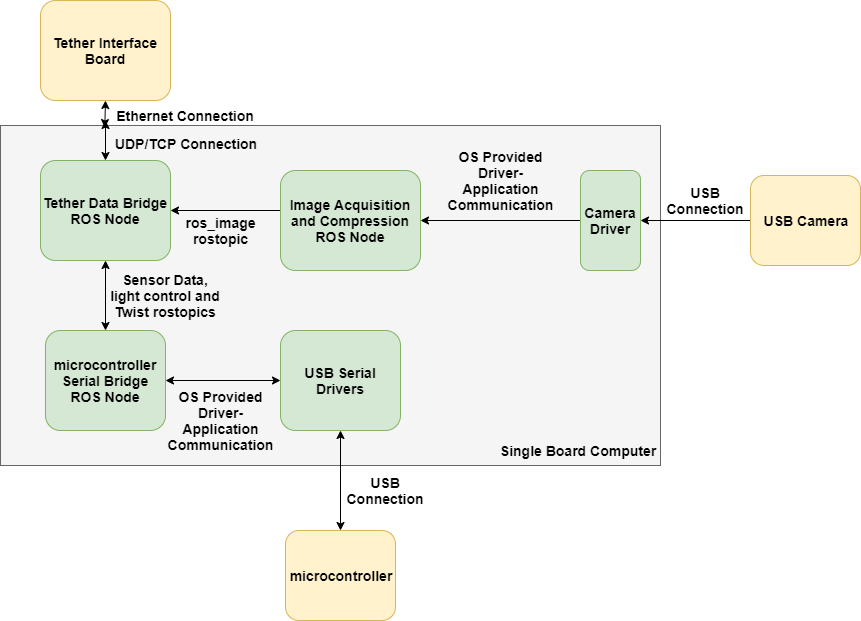
\includegraphics[scale=0.45]{SingleBoardComputerSoftware.png}
    \caption{Single Board Computer Software Interface Diagram}
    \label{fig:Single Board Computer Software Interface Diagram}
\end{figure}
\FloatBarrier

Within figure \ref{fig:Single Board Computer Software Interface Diagram}, The interfaces between each software component can be seen. All data retrieved from the microcontroller and USB camera will interface with their respective hardware drivers before sending each given data stream to ROS nodes the subscribe to the ROS topic in question. 

\subsection{Base Station Domain Software Interfaces}
The Base Station domain will have software interfaces to allow for data acquisition from the Xbox Controller, and software interfaces to allow for communication between the base station raspberry pi and the base station tether interface board. There will also be an API provided by a flash back end application to allow for the front end web application to communicate with the back end. The back end application will have software interfaces for communicating the the MongoDB database instance. All of these interfaces allow the fulfilment of the required functionality needed to control and monitor the ROV during the duration of the dive. Figure \ref{fig:Base Station Software Domain} depicts the high level software interfaces for the base station software domain.

\begin{figure}[!ht]
    \centering
    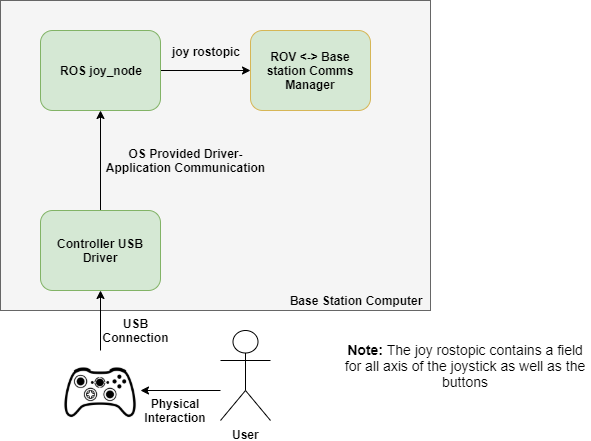
\includegraphics[scale=0.45]{UserInputCollection.png}
    \caption{User Input Collection Software Interface Diagram}
    \label{fig:User Input Collection Software Interface Diagram}
\end{figure}
\FloatBarrier

Figure \ref{fig:User Input Collection Software Interface Diagram} in this section depicts the software interfaces between the software components involved in user input collection via the Xbox controller. Data obtained from the Xbox controller will be published to any subscribing nodes via the ROS joy topic. It will likely be the case that the only node requiring this information in this phase will be the ROV<->Base station communication manager. 

\begin{figure}[!ht]
    \centering
    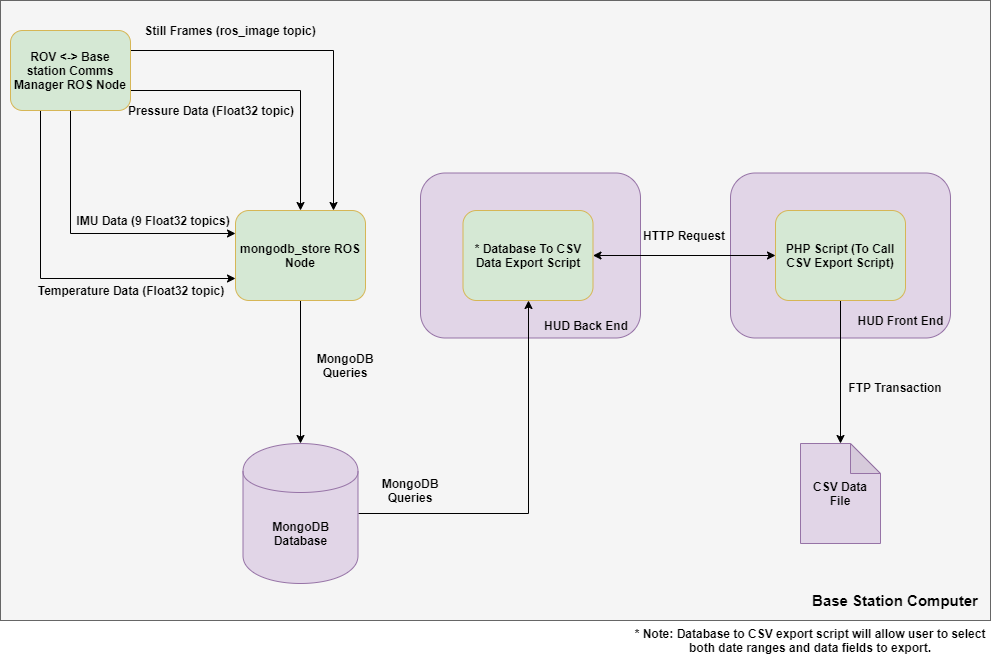
\includegraphics[scale=0.45]{DataArchival.png}
    \caption{Data Archival Software Interface Diagram}
    \label{fig:Data Archival Software Interface Diagram}
\end{figure}
\FloatBarrier

Figure \ref{fig:Data Archival Software Interface Diagram} in this section depicts the software interfaces between the various software components involved in the archiving of mission data into a MongoDB database instance, and the subsequent software required to retrieve that data at a later time. The MongoDB_store ROS node allows for data streams via ROS topics to be aggregated into a database in a time-series manner without an issue.

\begin{figure}[!ht]
    \centering
    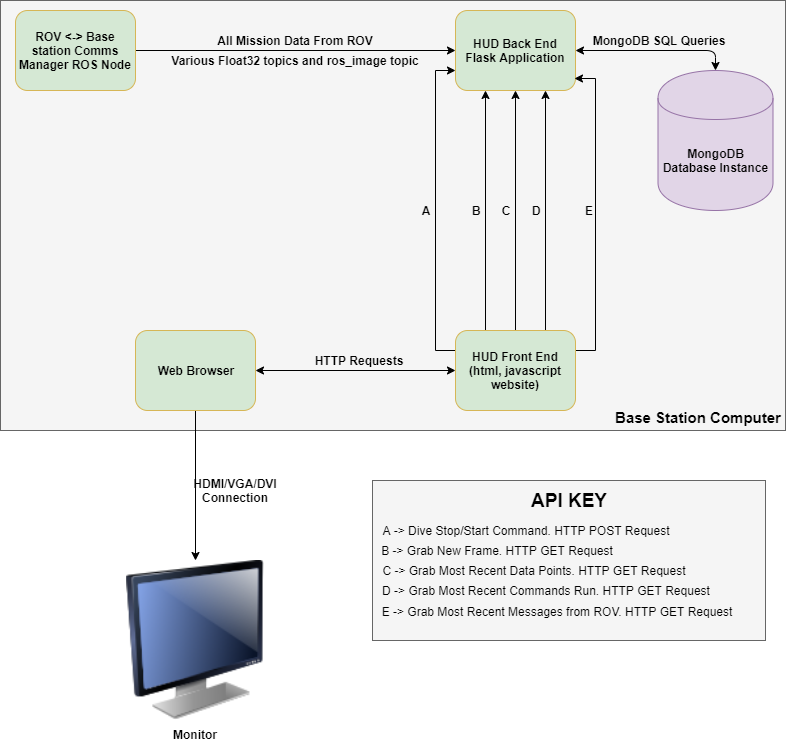
\includegraphics[scale=0.50]{HUDGUIManager.png}
    \caption{Software Interface for Main GUI Page Management}
    \label{fig:Software Interface for Main GUI Page Management}
\end{figure}
\FloatBarrier

Figure \ref{fig:Software Interface for Main GUI Page Management} in this section depicts the software interface required to support the main page of the HUD interface seen in \ref{fig:Main HUD Page Mockup View}. An API exposed within the back end flask application allows for the front end to request new frames, new mission data points, messages from the ROV, and a list of most recently run commands.  

\begin{figure}[!ht]
    \centering
    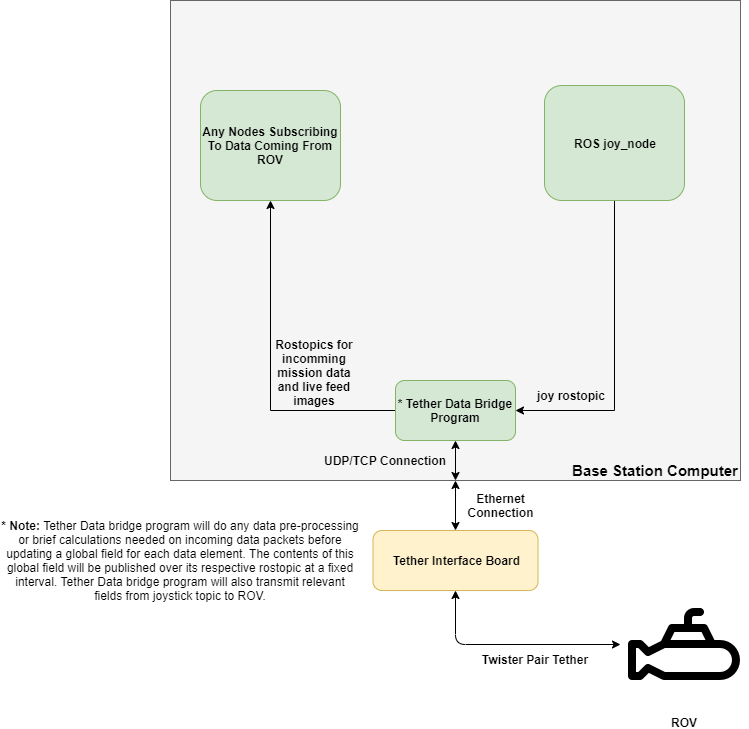
\includegraphics[scale=0.45]{ROVBaseStationCommsManager.png}
    \caption{Software Interfaces For The Base Station Communications Manager}
    \label{fig:Software Interface Base Station Communications Manager}
\end{figure}
\FloatBarrier

Figure \ref{fig:Software Interface Base Station Communications Manager} in this section depicts the base station communications manager software interface diagram. All data coming up the tether from the ROV is distributed to the rest of the system via rostopics through the tether data bridge program node. Data from the Xbox controller will be sent to the ROV via the joy rostopic through the tether data bridge program. Dive start and stop commands collected in the front end HUD interface seen in figure \ref{fig:Main HUD Page Mockup View} will be sent to the ROV through the back end via the tether data bridge program node.   



\subsection{Stimulus/Response Sequences}
This section outlines the Teensy micro-controller stimulus state diagram. This diagram outlines the looping structure that the micro-controller will perform at a fixed rate to ensure all data collected will be able to be retrieved by the rest of the system, and that they system can actuate the lighting controller and motor controllers in a responsive manner. Figure \ref{fig:Teensy Micro-Controller State Diagram} in this section outlines this state diagram.

\begin{figure}[!ht]
    \centering
    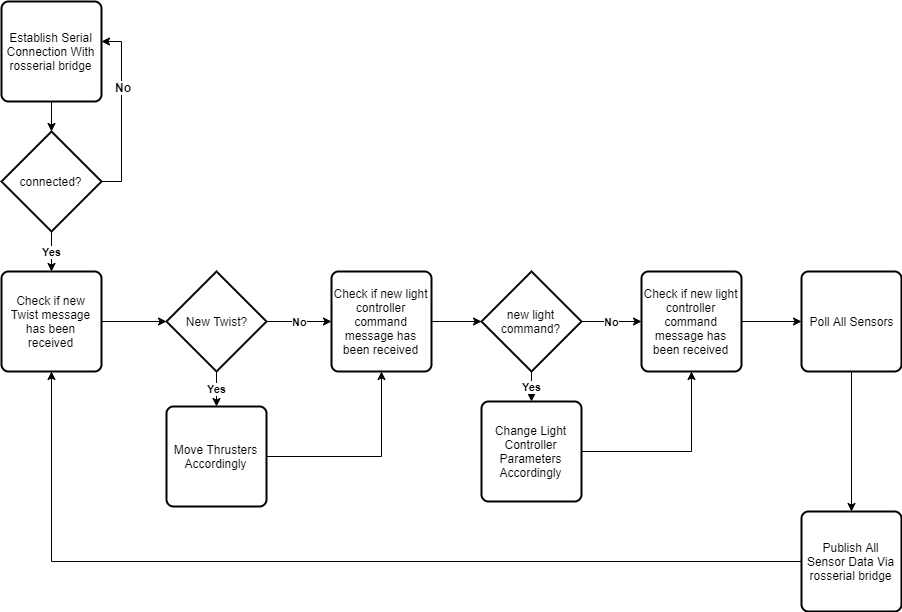
\includegraphics[scale=0.50]{microcontrollerStateDiagram.png}
    \caption{Teensy Micro-Controller State Diagram}
    \label{fig:Teensy Micro-Controller State Diagram}
\end{figure}
\FloatBarrier



\end{document}
